\chapter{Benutzeroberfläche}\label{cha:interface}

Dies Kapitel beschreibt das grundlegende  Konzept der Benutzeroberfläche, wie sie von \textsf{XCSoar} benutzt wird und ist als erste Übersicht zu verstehen. Mehr Details werden in den folgenden Kapiteln erörtert.

\begin{center}
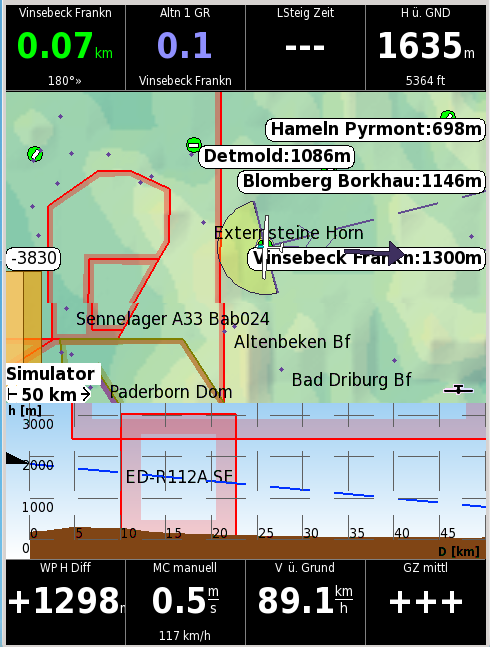
\includegraphics[angle=0,width=0.75\linewidth,keepaspectratio='true']{figures/plain.png}
\end{center}

Die  \textsf{XCSoar} Anzeige besteht aus mehreren Teilen:
\begin{description}
\item[\p{Kartenanzeige}] Die größte Fläche des Bildschirmes wird vom GPS-moving map beansprucht.
Wichtige Symbole, welche Informationen des Segelflugrechners darstellen, werden auf dieser Karte
eingeblendet (z.B. die Über/Unter Gleitpfad-Pfeile am linken Rand oder das Thermik-Höhenband).
Einige Icons und Textinformationen  erscheinen  (bei Bedarf) am unteren Rande des Displays,
welche über den Zustand des Rechners (verbunden mit GPS, Kurbelmodus, Endanflugmodus) etc.\  informieren.
%
\item[\p{{\InfoBox}en}] Eine bislang nur rechteckige Anordnung von sogenannten Info-Boxen, welche mit diversen Angaben, wie zum Beispiel Geschwindigkeit über Grund,
Höhe, MC Cready, geschätzte Zeit zum nächsten Wegpunkt usw. gefüllt ist, kann entweder am oberen und unteren Rand, rechts oder links,
oder auf der rechten Seite des Displays (im Quer- bzw. landscape-Modus) angezeigt werden. Bislang sind diese Anordnungen fix, in zukünftigen Versionen ist jedoch angestrebt, diese Infoboxen auch frei verschiebbar auf dem Display anordnen zu können.
%
hier werden diejenigen Werte, die der Benutzer vorher ausgewählt  hat und von \textsf{XCSoar} bzw. angeschlossenen Geräten ausgewertet werden, angezeigt.
%
\item[\p{Anzeigen}] Anzeigen stellen Instrumenten Displays dar (z.B. ein Vario). Alle Anzeigen sind optional und einige
haben lediglich informellen  Character, wenn \textsf{XCSoar} an ein unterstütztes Instrument angeschlossen ist.
%
\item[\p{Button Beschriftungen and Menüs}] Hardware-Knöpfe und die Wippe des Gerätes, auf dem \textsf{XCSoar} läuft, können benutzt werden, um Menüs bzw.\ Hauptmenüs aufzurufen, welche typischerweise den Hardwareknöpfen und /oder der Wippe fix zugeordnet sind. Dies erlaubt mitunter einen schnelleren Zugriff als das Bedienen allein des berührungsempfindlichen Bildschirmbereiches ("TouchScreen").
Falls das entsprechende Gerät über einen solchen TouchScreen verfügt (nahezu alle bis auf \al), können alle Menüs auch
hierüber geöffnet und bedient werden. Diese Buttons sind in schwarzem Text auf hellgrünem/grauen Hintergrund gestaltet.
%
\item[\p{Status Meldungen}] Hinweise zum Status des Fluges und auch des Flugzeuges  (z.B.\ Annäherung an einen Luftraum, vergessenes Fahrwerk, Startbestätigung bei Überfliegen der Start/Ziellinie etc\dots ) wird in einer Textbox  über dem Bildschirm eingeblendet.
Dieser Status Meldungen werden angezeigt, um detaillierte, wichtige Informationen zu geben, wenn gewisse, zum Teil konfigurierbarer Ereignisse, auftreten.
%
\item[\p{Dialog Fenster}] Die -größeren- Dialogfenster enthalten normalerweise Grafiken und Buttons. Diese werden verwendet, um dem Piloten  detaillierte Daten bezüglich Wegpunktdetails, Statistik und Analyse des bisherigen Fluges, Polaren etc\dots  zu übermitteln.

\item[\p{Hauptmenü}] das Hauptmenü wird entweder über einen Doppelklick auf die Bildschirmoberfläche oder aber über Gesten \gesture{Runter - Hoch} aufgerufen.

   Wenn die erscheinenden Buttons nicht innerhalb einer gewissen (einstellbaren) Zeit  betätigt  werden, verschwinden sie von sich aus wieder, um die Kartendarstellung des weiteren Fluges nicht zu behindern.
\end{description}

Die Bedienung von \textsf{XCSoar} ist auf verschiedene Wege möglich:

\begin{itemize}
\item Anklicken eines speziellen Kartenelements
\item Anklicken einer InfoBox und anschließend den Bildschirmmenüs
\item Benutzen einer "Geste", z.B. Zeichnen eines Striches von links nach rechts auf dem TouchScreen
 (siehe dazu Kap.~\ref{sec:gestures} weiter unten).
\item "Verschieben" (dragging) des Bildschirms (berühren und verschieben auf dem TouchScreen unter Fingerdruck).
\item Drücken der Hardware-Knöpfe des  Gerätes.
\item Drücken der Wippe des Gerätes.
\item Drücken  oder Schalten  an einem an \textsf{XCSoar} angeschlossenen Gerät.
\end{itemize}

Je nachdem, welcher Hardware bzw.\ welches Gerät mit \textsf{XCSoar}  benutzt wird, stehen nicht alle dieser Methoden zur Verfügung. Die Belegung der jeweiligen Hardware-Knöpfe können daher unterschiedlich sein.

Bei der \textsf{PC}-Version von \textsf{XCSoar} ist das Anklicken eines Bildschirmelements es mit der Maus identisch der Berührung mittels Touchscreen.

Da der \al nicht über einen TouchScreen verfügt, ist hier die Belegung der Menüs und Elemente grundlegend anders und wird über die dort vorhanden Hardware-knöpfe und Drehgeber vorgenommen.

 \newpage
 \section{Grundlegende Layouts von\textsf{XCSoar}}
 \textsf{XCSoar} läßt sich von der Oberfläche her extrem flexibel anpassen, je nach Geschmack des Benutzers. 
 Ich will hier lediglich vier unterschiedliche Darstellungen zeigen, welche allesamt im Konfigurationsmenü eingestellt werden können. 

 \begin{center}
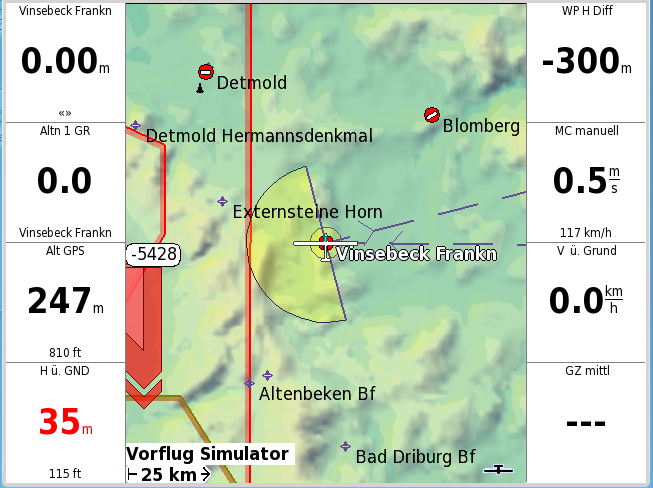
\includegraphics[angle=0,width=0.45\linewidth,keepaspectratio='true']{figures/map-outfit2.png}\quad
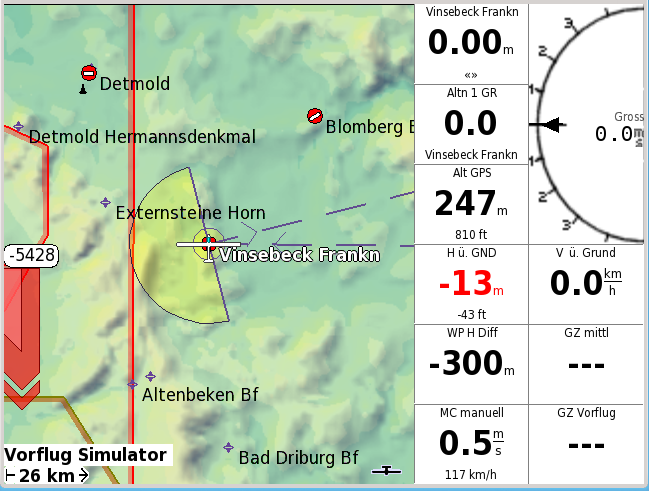
\includegraphics[angle=0,width=0.45\linewidth,keepaspectratio='true']{figures/map-outfit3.png}\vspace{1em}
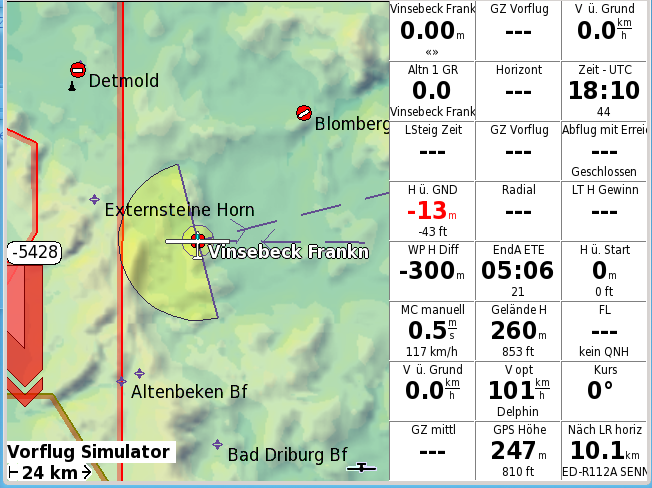
\includegraphics[angle=0,width=0.45\linewidth,keepaspectratio='true']{figures/map-outfit4.png}\quad
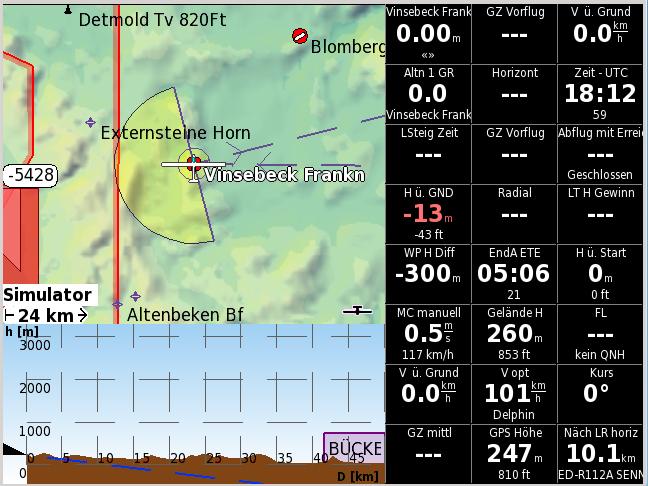
\includegraphics[angle=0,width=0.45\linewidth,keepaspectratio='true']{figures/map-outfit5.png}\vspace{1em}
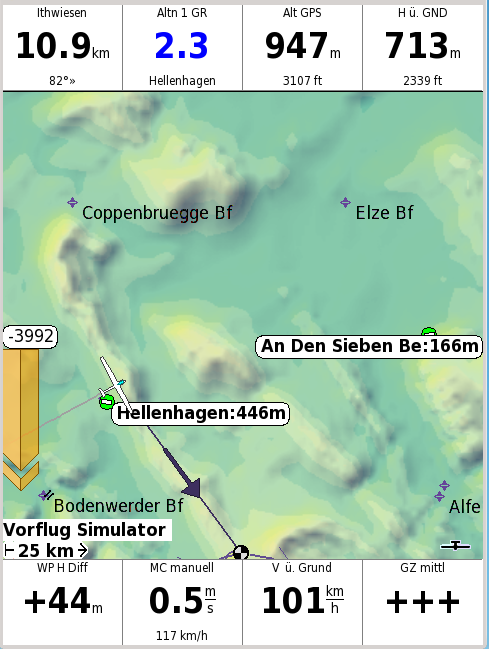
\includegraphics[angle=0,width=0.45\linewidth,keepaspectratio='true']{figures/map-outfit1.png}\quad
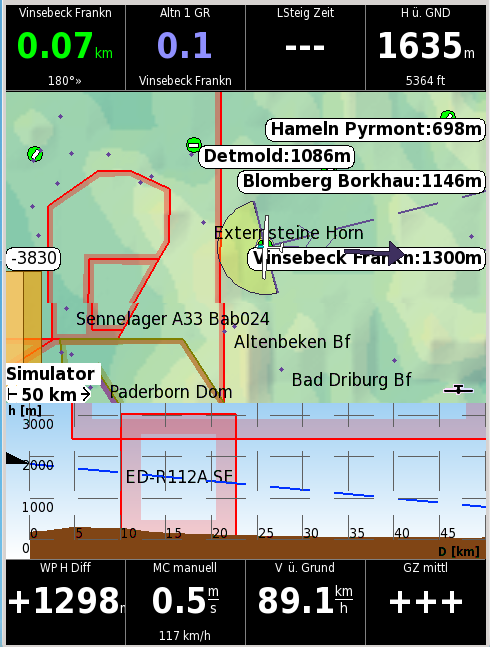
\includegraphics[angle=0,width=0.45\linewidth,keepaspectratio='true']{figures/map-outfit6.png}
\end{center}
Ob hochkant, quer, quadratischt schwarz oder weiß, mit Vario oder ohne, auch komplett ohne Infoboxen - alles möglich.
Die Einstellungsvarianten mögen auf den ersten Blick schier unübersichtlich sein, innerhalb weniger Tage oder Flüge jedoch habt ihr mit Sicherheit Eure Lieblingskonfiguration gefunden.


Ich beschränke mich in diesem Handbuch  grundsätzlich auf die hocjhkant (Portrait) Darstellung, da fats alle älteren PDA nur für diese geeignet erscheinen. Bei moderneren Android Geräten mag dies anders ein. Kann ja jeder machen wie er lustig ist.
   
 \newpage\section{Button-Beschriftungen und -Menüs}
Das Button-Menü besteht aus einem Satz von Buttons und Menüs und ist wird -bis auf die o.g. genannten Ausnahmen- mittels des TouchScreens aufgerufen (Doppelklick auf die berührungsempfindliche Oberfläche).

Die Benutzung der Buttons und des Button-Menüs  stellt die bevorzugte Art der Interaktion mit \textsf{XCSoar} dar.

\begin{center}
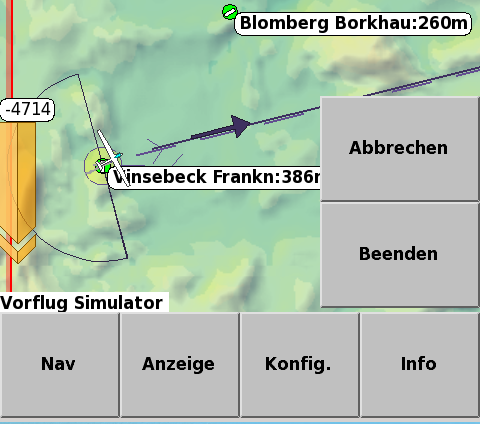
\includegraphics[angle=0,width=0.75\linewidth,keepaspectratio='true']{figures/buttonmenu.png}
\end{center}

\subsection*{Grundlegende Info zur Bedienoberfläche}
Das Menü ist in vier Hauptgruppen mit hoffentlich aussagekräftigen Namen (\textbf{Nav}, \textbf{Anzeige}, \textbf{Konfig.} und \textbf{Info}) unterteilt, welche diverse Untermenüs besitzen. Das spezielle Layout hängt vom jeweils benutzten Gerät ab und kann ebenso vom Bediener angepaßt werden. \textbf{Beenden} und \textbf{Abbrechen} vertseht sich wohl von slebst. 

 \textsf{XCSoar} kann ebenso über an das Gerät angeschlossene externe Eingabegeräte wie Joysticks, externe Tastaturen, game-pads und Multifunktionsgriffe bedient werden. Die hierüber aufzurufenden Funktionen können in großem Rahmen eben falls frei konfiguriert  werden.


Beim  \al  gibt es vier Hauptmenüs, welche durch Drücken auf die Knöpfe an der linken Seite aufgerufen werden können. 

Sowie ein Menü aktiviert wurde, erscheinen Untermenüs mit entsprechenden Beschriftungen über der unteren Druckknopfreihe. 
Hiermit kann man sich dann durch die entsprechenden Menüs und Funktionen weiter hindurchmanöverieren. 
Auf der letzten Seite eines jeden Menüs erscheint wieder der Menü-Knopf, mit dem man schließlich wieder auf den 
Bildschirm zurückkommt und alle Menüs verschwinden wieder vom Schirm. 
 


Auf dem \textsf{PC} werden diese Hauptmenü-Funktionen über die Ziffertasten 1, 2, 3 und  4 aufgerufen. Die Tasten 6, 7, 8, 9 und  0 sind dabei mit den
entsprechenden Untermenü-Funktionen der horizontal bzw.\ vertikal angeordneten Reihe von Buttons  zugeordnet.

Bei der PDA Version können die Hauptfunktionen direkt über die vier Hardware-Knöpfe über/unter (je nach Gerät) neben der Schaltwippe aufgerufen werden.

Falls ein Menü aufgerufen wird und nach einer gewissen Zeit keinerlei Eingabe mehr erfolgt, wird das angewählte Menü automatisch wieder geschlossen.  Diese Verzögerungszeit ist frei definierbar.  Auf dem \textsf{PC} kann die ESC- Taste hierzu benutzt werden, beim  \al wird hierzu der PWR/ESC- Knopf benutzt.

Wenn die Menü-Buttons grau erscheinen, ist die entsprechende Funktion nicht verfügbar.

So ist zum Beispiel der Button \textcolor{white}{\button{Wegpunkt Liste}} grau hinterlegt und die Schrift weiß gefärbt, falls keine Wegpunkt-Liste (besser: keine Wegpunkt-Datei) zur Verfügung steht oder geladen ist.

Einige der Menü-Buttons sind mit dynamischem Text versehen, d.h. die Beschriftung ändert sich entsprechend des Zustandes (gedrückt/nicht gedrückt). Folgendes Verhalten ist hierbei grundlegend festgelegt:


\textbf{Die Beschriftung des Buttons zeigt an,\textcolor[rgb]{0.72,0.03,0.20}{ was geschehen wird}, wenn er \achtung gedrückt wird, er zeigt also nicht den aktuellen Zustand an!}\index{Schaltflächen!Anzeigeverhalten}

Wird zum Beispiel auf der Schaltfläche  \button{MC Auto} angezeigt, dann wird ein Klick hierauf   'Auto
McCready' einschalten, und die Beschriftung wechselt zu  \button{MC Manuell}.
In der unten aufgelisteten Liste sind die Standard Beschriftungen aufgeführt.

\subsection*{Übersicht der Menüs}\index{Menü!Übersicht}
Im Folgenden wird beschrieben, wie das Menü allgemein aufgebaut ist.
Dies gilt für alle Plattformen (\textsf{PC}, Android, \al PDA, etc\dots

Die entsprechenden Funktionen werden in nachfolgenden Kapiteln ausführlicher beschrieben.

\textsf{\al}:

Die vier primären Menübuttons (Hauptmenü) werden beim \al durch Drücken der vertikal angeordneten Knöpfe an der linken Seite wie folgt von unten nach oben aktiviert:

\begin{jspecs}
\item[\button{Nav}]      Kontrolle und Einstellungen bezüglich Navigation, hauptsächlich gedacht für Tasks (Aufgaben).
\item[\button{Anzeige}]  Einstellungen der Anzeige von \textsf{XCSoar}
\item[\button{Konfig.}]  Konfiguration von \textsf{XCSoar}, angeschlossener Geräte,
                                      Einstellungen während des Fluges (Wind, Ballast, MC etc.\
\item[\button{Info}]     Aufruf diverser Informations Fenster,  Checkliste, Lufträume, Wetter etc.\
\end{jspecs}

In der \textsf{\textsf{PC}}-Version werden hierfür die Tasten  1, 2, 3 und 4 verwendet.

\subsection*{Navigationsmenü (Nav)}\index{Navigations-Menue}\index{Menü!Navigation}
\jindent{\bmenus{Aufgabe}}{ Blendet Aufgabenverwaltung und - Rechner ein. }
\jindent{\bmenut{Vorheriger}{Wegpunkt}}{ Wählt den vorherigen Wegpunkt innerhalb der Aufgabe an. }
\jindent{\bmenut{Nächster}{Wegpunkt}}{ Wählt den nächsten Wegpunkt innerhalb der Aufgabe an.}
\jindent{\bmenut{Wegpunkt}{Liste}}{ Zeigt die Wegpunkt - Auswahl an.}
\jindent{\bmenus{Alternativen}}{ Zeigt eine  Schnellauswahl-Liste der nahesten landbarer und erreichbarer Plätze in der Nähe an.}
%
%
%
\jindent{\bmenut{Aufgabe}{Abbruch}}{ Bricht die Aufgabe ab und geht über in den "Lustflug-Modus".}
\jindent{\bmenus{Gehezu}}{ Blendet die Wegpunkt-Auswahl 1ein und aktiviert den "Gehezu"-Modus für den ausgewählten Wegpunkt. }
\jindent{\bmenus{Target}}{ Zeigt den Target-Dialog. Entscheidend für AAT-Aufgabe. Hier können u.a. AAT-Wegpunkte verschoben werden. }
\jindent{\bmenut{Wegpunkt}{Details}}{ Blendet Details zum aktuell gewählten Wegpunkt ein.}


\subsection*{Anzeigemenü (Anzeige)}\index{Anzeige-Menue}\index{Menü!Anzeige}
\jindent{\bmenut{Zoom}{herein}}{ Zoomt die Karte herein (Kartenausschnitt kleiner, mehr Details. }
\jindent{\bmenut{Zoom}{heraus}}{ Zoomt  die Karte heraus (Kartenausschnitt größer,weniger Details. }
\jindent{\bmenut{Zoom}{Auto}}{ Schaltet zwischen  Zoom Auto und  Zoom Manuell hin und her. }
\jindent{\bmenut{Marke}{Setzen}}{ Setzt einen Marker der aktuellen Position auf der Karte. }
\jindent{\bmenut{Verschieben}{Ein}}{ Schaltet den Verschiebe-Modus der Karte ein. }
%
%\jindent{\bmenut{Beschriftungen}{Aufgaben\& Landeplätze}}{ Blendet die Beschriftungen der Wegpunkte innerhalb Aufgaben ein oder aus.. }
\jindent{\bmenud{Beschriftungen}{Aufgaben}{\& Landeplätze}}{ Blendet die Beschriftungen der Wegpunkte innerhalb Aufgaben ein oder aus.. }
\jindent{\bmenut{Spur}{Kurz}}{ Schaltet die Spur des bisherigen Fluges (kurz, lang, aus). }
\jindent{\bmenut{Gelände}{Aus}}{ Schaltet die Darstellung de Geländes auf der Karte ein oder aus. }
\jindent{\bmenut{Topo.}{Aus}}{ Schaltet die Topologie ein oder aus. }
\jindent{\bmenut{Info}{Auto}}{ Schaltet die Infoboxen (Kurbeln, AAT, Endanflug, Auto). }
%
%
%
\subsection*{Konfigurationsmenü (Konfig.\ )}\index{Konfig-Menue}\index{Menü!Konfig}
\jindent{\bmenut{MC}{$+$}}{ McCready größer. }
\jindent{\bmenut{MC}{$-$}}{ McCready kleiner. }
\jindent{\bmenut{MC}{Auto}}{ Schaltet zwischen McCready Auto oder und McCready manuell. }
\jindent{\bmenut{Flug}{Einstellungen}}{ Zeigt das Flug-Einstellungsfenster  (Mücken, Ballast, QNH). }
\jindent{\bmenut{Wind}{Einstellung}}{ Ruft das Windeinstellungsmenü auf.}
%
%
%
\jindent{\bmenus{Vario}}{ Kontrolle des Vega - Varios, dies enthält ein Untermenü.  Nur wählbar, wenn auch ein Vega angeschlossen ist. }
\jindent{\bmenut{System}{Einstellungen}}{ Öffnet die \textsf{XCSoar}-System-Einstellungen. Hierunter liegen 21 weitere Dialogfenster zur kompletten Konfiguration \textsf{XCSoar}s. }
\jindent{\bmenut{Luftraum}{Einstellungen}}{ Öffnet den Luftraum-Dialog. }
\jindent{\bmenut{Logger}{Start}}{ Schaltet den internen \textsf{XCSoar}- IGC-Logger an oder aus.. }
\jindent{\bmenus{Wiedergabe}}{ Startet das Wiedergabe-Fenster aufgezeichneter Flüge. }
%
\jindent{\bmenut{Roh}{Logger}}{ Schaltet den NMEA-Rohdaten-Logger ein oder aus (nur benutzt zur Entwicklung/Debuggen von \textsf{XCSoar}). }
\jindent{\bmenus{NMEA}}{ Öffnet den NMEA (z.B. GPS-Anschluß) Dialog. }
\jindent{\bmenus{Flugzeug}}{ Öffnet den Dialog zur Eingabe von flugzeugspezifischen Details. }
%
%
%
\subsection*{Informations Menü  (Info)}\index{Info - Menue}\index{Menü!Info}
\jindent{\bmenus{FLARMRadar}}{ Öffnet das Flarm-Radar-Fenster (Nur, wenn Flarm angeschlossen und erkannt) }
\jindent{\bmenut{METAR}{TAF}}{ Zeigt das METAR/TAF Fenster. }
\jindent{\bmenut{Naher}{Luftraum}}{ Zeigt die Details des nächstgelegenen Luftraumes. }
\jindent{\bmenut{Check}{Liste}}{ Öffnet die Checkliste, falls vorhanden}
\jindent{\bmenus{Analyse}}{ Öffnet den Analyse/Statistik-Dialog. }
%
\jindent{\bmenus{Status}}{ Öffnet den Status-Dialog. }
\jindent{\bmenus{Weather}}{ Öffnet das Wetter-Dialog-Fenster. }
\jindent{\bmenut{Team}{Code}}{ Einblendung des TEAM-Code Dialoges.}
\jindent{\bmenut{FLARM}{Details}}{ Öffnet das FLARM-Detail-Fenster.}
\jindent{\bmenus{Zentrierhilfe}}{ Öffnet die Zentrierhilfe.}
%
\jindent{\bmenus{Mitwirkende}}{ Zeigt Versionsnummer und eine Reihe der Mitwirkenden an \textsf{XCSoar} an. }
\jindent{\bmenut{Naher}{Wendepunkt}}{ Zeigt Details des nächst gelegenen Wegpunktes an. }
\jindent{\bmenut{Wiederhole}{Meldung}}{ Wiederholt die zuletzt ausgegebene Meldung \textsf{XCSoar}s. }
%
%
%
\subsection*{Variometer-Untermenüs (Vario) des Konfigurationsmenüs (Konfig.\ )  }
Die Funktionen dieses Menüs sind ausschließlich anwählbar, wenn das VEGA Vario als Gerät an \textsf{XCSoar} angeschlossen ist.
\begin{center}

\end{center}
\jindent{\bmenut{Airframe}{Switches}}{ Displays airframe switch values. }
\jindent{\bmenut{Setup}{Audio}}{ Adjusts volume of sounds produced by \textsf{XCSoar} as well as certain speech announcements by the Vega intelligent variometer. }
\jindent{\bmenut{Manual}{Demo}}{ Activates Vega variometer manual tone demo. }
\jindent{\bmenut{Setup}{Stall}}{ Opens Vega stall monitor setup dialog. }
\jindent{\bmenus{Accel}}{ }
\jindent{\bmenut{ASI}{Zero}}{ Zeros the airspeed indicator. }
\jindent{\bmenut{Accel}{Zero}}{ Levels/zeros the accelerometers. }
\jindent{\bmenus{Store}}{ Stores Vega settings to EEPROM. }
\jindent{\bmenut{Cruise}{Demo}}{ Activates Vega variometer cruise tone demo. }
\jindent{\bmenut{Climb}{Demo}}{ Activates Vega variometer climb tone demo. }
\subsection*{Verschieben-Untermenü des Anzeige-Menüs}
\jindent{\bmenut{Verschieben}{aus}}{ Schaltet Verschiebemodus aus. }
\jindent{\bmenut{Zoom}{herein}}{ Zoomt Karte herein. }
\jindent{\bmenut{Zoom}{heraus}}{ Zooms Karte heraus. }
\jindent{\bmenut{Naher}{Wegpunkt}}{ Zeigt das Wegpunkt-Detail Fenster, oder aber, falls die Karte verschoben wurde, das Wegpunkt-Detail Fenster zu jenem Wegpunkt, an dem sich das Fadenkreuz (sichtbar beim Verschieben, immer in der Mitte der Karte), befindet. }
\subsection*{Standard-Buttons}\index{Buttons!Standard}
Wenn keinerlei Menü aktiv ist, (der sog.\ \textsl{default-mode}) dann sind beim \al den horizontalen Knöpfen die folgenden Funktionen zugeordnet. In der oberen Reihe die \textsf{PC}-Tasten, in der unteren Reihe die \al-Tasten.
Unten die entsprechende Standard-Funktionsbelegung:
\begin{center}
\begin{tabular}{c c c c c}
 6 & 7 & 8 & 9 & 0 \\
 F5 & F6 & F7 & F8 & F9 \\
\smenut{Flug}{Einstellung} & \smenut{Task}{Calc} & \smenut{Task}{Edit} &
\smenut{Arm}{Advance} & \smenut{Marker}{setzen} \\
\end{tabular}
\end{center}

Wenn der ESC-Knopf des \al kurz gedrückt wird, erscheint die Beschreibung der Knöpfe.
Bei allen anderen Geräten / Plattformen wirken die cursor-Tasten wie folgt:


\begin{jspecs}\index{Buttons!\al}
\item[\p{Hoch Taste}] Zoom herein
\item[\p{Runter Taste}] Zoom hinaus
\item[\p{Links Taste}] Nächster InfoBox-Set
\item[\p{Rechts Taste}] Letzter InfoBox-Set
\item[\p{Enter}] Bestätigen/Löschen von Status-Mitteilungen oder aber Flarm-Meldungen unterdrücken, wenn diese erscheinen und keine Warnung aktiv ist
\end{jspecs}
Der Drehknopf des \al  ist im default-mode wie folgt belegt:


\begin{jspecs}
\item[\p{Äußerer Knopf gegen Uhrzeigersinn}] Zoom herein
\item[\p{Äußerer Knopf im Uhrzeigersinn}]  Zoom heraus
\item[\p{Innerer Knopf gegen Uhrzeigersinn}] (Nicht belegt)
\item[\p{Innerer Knopf im Uhrzeigersinn}] (Nicht belegt)
\item[\p{Drücken des Knopfes}] Bestätigen von Status Meldungen und Luftraum Warnungen/Hinweisen
\end{jspecs}




In Dialog Fenster sind den Drehknöpfen des \al folgende , Cursor-ähnliche Funktionen zugewiesen:


\begin{jspecs}
\item[\p{Äußerer Knopf gegen Uhrzeigersinn}] Cursor hoch
\item[\p{Äußerer Knopf im Uhrzeigersinn}] Cursor runter
\item[\p{Innerer Knopf gegen Uhrzeigersinn}] Cursor links
\item[\p{Innerer Knopf im Uhrzeigersinn}] Cursor rechts
\item[\p{Drücken des Knopfes}] Bestätigen/OK-Taste
\end{jspecs}


Beim \al können alternativ die folgenden Knöpfe entlang des Gehäuserandes für die Navigation innerhalb von Dialogen benutzt werden:

Der F4-Knopf kann innerhalb von Dialogen als alternative zur ENTER-Taste (Drücken des Drehknopfes) benutzt werden.
F6 und F7 können benutzt werden um die nächste bzw.\ letzte Seite innerhalb von Dialogseiten anzuwählen.
\subsection*{Dynamische Menübeschriftungen}\index{Menü-Beschriftungen}
Die meisten Menüs haben dynamische Beschriftungen, um klarer hervorzuheben, welche Aktion diesem Menü zugeordnet ist, wenn der jeweilige Button bedient wird.

Falls ein Menü oder Button grau hinterlegt ist, so steht diese Funktion zum jeweiligen Zeitpunkt \emph{nicht} zur Verfügung und ein Klick darauf bewirkt gar nichts.

Folgende Konvention zur Belegung bzw. Beschriftung der Buttons und Menüs wird  innerhalb \textsf{XCSoar} verwendet:

Beispiel:

Erscheint z.B.:  "Licht an'' als Beschriftung, so  wird das Licht \emph{an}geschaltet und  es erscheint dann als Beschriftung z.B. "Licht aus".  Ein erneute Drücken schaltet dann das Licht wieder \emph{aus}.

Stehen mehrere Funktionen eines Knopfes zur Verfügung, (z.B.\ zusätzlich noch "Licht gedimmt", dann kann durch Drücken des Buttons zyklisch durch diese Funktionen durchgewählt werden:


\begin{center}
"Licht an'' $\rightarrow$ "Licht gedämmt'' $\rightarrow$ "Licht aus'' $\rightarrow$" Licht an" $\rightarrow$ "Licht gedämmt'' und so weiter\dots
\end{center}

Eine Auswahl von dynamisch beschrifteten Buttons ist als Beispiel hier unten aufgelistet:

\begin{description}
\item[\button{Nächster Wendepunkt}]
  Grau, wenn keine  Aufgabe aktiv ist, oder aber wenn der nächste Wendepunkt gleich dem Zielpunkt (also dem letzten Wegpunkt) ist.

 Wenn der nächste Wegpunkt gleich dem Ziel ist, dann erscheint " Wendepunkt Ziel''.
\item[\button{Letzter Wendepunkt}]
  Grau, wenn keine  Aufgabe aktiv ist, oder aber wenn der vorherige Wendepunkt gleich dem Startpunkt ist und es keine verlegten Startpunkte gibt. .

  Falls verlegte Startpunkte vorhanden sind und der aktive Wendepunkt gleich dem Start ist, wird "zyklischer Start" angezeigt um aus den diversen Startpunkten einen entsprechenden auszuwählen.

Wenn der aktive Wegpunkt gleich dem ersten Wegpunkt nach dem Start ist, dann erscheint  "Wendepunkt Start''.
\item[\button{Beschriftungen}]
Angezeigt wird hierbei folgendes: " Beschriftung Aufgabe \& Landeplätze", "Beschriftung Keine", Beschriftung Alle.

\item[\button{Nächster Wendepunkt}]
 Grau,  wenn keine Wegpunkt-Datenbank hinterlegt ist.
 \item[\button{Vorheriger Wendepunkt }]
  Grau,  wenn keine Wegpunkt-Datenbank hinterlegt ist.
\item[\button{Wegpunktliste }]
  Grau,  wenn keine Wegpunkt-Datenbank hinterlegt ist.
\end{description}

\section{{\InfoBox}en}\index{InfoBoxen}

\textsf{XCSoar} stellt nahezu alle wichtigen Werte mittels  sog.\  {\InfoBox}en dar. 


Diese {\InfoBox}en können zu InfoBoxfenstern (s.u.) zusammengestellt werden und mit
\emph{gewissen Einschränkungen \footnote{In Planung ist, in kommenden Versionen einige oder alle 
InfoBoxen auch frei verschiebbar darzustellen}} beliebig auf dem Bildschirm plaziert werden. 
Die Informationen, welche in den  {\InfoBox}en dargestellt werden sollen,  können aus einer großen Anzahl (gelistet im Kapitel~\ref{cha:infobox}) ausgewählt werden.

Die mögliche Anzahl und das Layout \sketch{figures/infoboxes.png}der {\InfoBox}en  hängen von der Ausrichtung des Bildschirmes und von der Größe bzw. Auflösung des Bildschirms des entsprechende Gerätes ab. 

Für ein typisches 320$\times$240 Pixel-Display (Pocket-\textsf{PC} im "Hochkant"-Modus) stehen jeweils vier {\InfoBox}en am oberen und unteren Rand des Displays zur Verfügung. 
Im Querformat, sind neun {\InfoBox}en an der rechten Seite des Displays vorgesehen. Siehe Bild unten:

%\begin{center}
%\includegraphics[angle=0,width=0.35\linewidth,keepaspectratio='true']{figures/infoboxes.png}
%\end{center}

%\begin{quote} \smenus{Konfig.\ }\blink\smenus{Konfig.\  }\blink%
%\smenut{System}{Einstellung}\blink\seite{19}
%\end{quote} Unterpunkt  "InfoBox Geometrie"\index{Infbox!Seiten!Anordnung}

\subsection*{Bildschirmanzeige-Modi / InfoBox-Seiten}\index{InfoBoxen!Seiten}

\textsf{XCSoar} gestattet dem Piloten einen ganzen Satz an individuell belegten Infobox-Seiten zu erstellen.
Dies dient dazu, bestimmte Werte, die zum Beispiel vor allem beim Kurbeln  benötigt werden übersichtlich und schnell darzustellen.
Ein anderer Satz an Infoboxen könnte zum Beispiel für den Endanflug oder aber während Wettbewerbsaufgaben erstellt und angezeigt werden.

\textsf{XCSoar} so kann so konfiguriert werden, daß es automatisch auf die jeweilige Seite umschaltet, oder aber ein manuelles Umschalten erforderlich ist. Der Name der aktuellen InfoboxSeite kann ganz unten links am Rande der Karte abgelesen werden.

Es ist ebenfalls möglich, überhaupt keine Infoboxen auf der Karte darzustellen, in diesem Fall erscheint ausschließlich die Landkarte mit Topologie bzw. Karte auf dem Bildschirm.

Um durch die diversen Infobox-Seiten hindurch zu schalten, kann der TouchScreen benutzt werden
\gesture{Rechts oder Links}. 

Auf PDA ist es ebenfalls möglich,  mittels der Schaltwippe  (nach rechts oder links) durch die diversen Seiten hindurch zu schalten.

\subsection*{Ändern von  {\InfoBox} Werten}\index{InfoBoxen!Werte Ändern}
(Dieser Abschnitt ist ausschließlich gültig, wenn ein Touchscreen oder eine Maus zur Verfügung steht.)

Einige {\InfoBox}-Werte können durch drücken auf den Touchscreen oder aber mit der Maus vom Piloten geändert.
Hierzu müssen die entsprechenden {\InfoBox}en  \emph{langanhaltend} gedrückt werden.
Ein kurzes Klicken reicht dazu nicht.  Nach dem loslassen erscheinen weitere {\InfoBox}en:

\begin{description}
\item[\button{Edit}]
Erlaubt dem Piloten den Wert der entsprechenden {\InfoBox} zu ändern (zum Beispiel den McCready Wert).

\item[\button{Setup}]
hiermit kann das Verhalten der entsprechenden {\InfoBox} geändert werden. Beispielsweise kann der McCready Wert von Auto auf Manuell geschaltet werden.
Weiterhin kann hier durch Klicken auf  \button{Setup InfoBox} innerhalb dieser {\InfoBox}  eine Liste mit allen verfügbaren {\InfoBox}en dargestellt werden, welche an dieser Stelle der InfoboxSeite erscheinen soll. hierzu erscheint ein Button "Infobox Einstellungen"

\item[\button{Schließen}] Na, was wohl\dots
\end{description}

{\InfoBox}en, deren Werte geändert werden können, sind zum Beispiel der McCready wert, oder aber die Windgeschwindigkeit und Richtung. Im Simulator-Modus, zählt auch die Höhe, sowie die Übergrundgeschwindigkeit hierzu.

\subsection*{Ändern von {\InfoBox}en}
{\InfoBox}en können entweder über das Konfigurationsmenü geändert werden 
\menulabel{\bmenut{Konfig.}{2/3}\blink\bmenus{System}} (ausführlich beschrieben in Kap.\ref{sec:interface-appearance})
oder durch einen länger anhaltenden Druck auf die entsprechende  {\InfoBox}, welche geändert werden soll.
 In diesem Fall erscheint ein Dialog mit allen verfügbaren {\InfoBox}en, aus denen die \menulabel{~~\button{Aussehen}\blink\button{Infobox Sets}}gewünschte ausgewählt werden kann.
 

\section{Status Meldungen}
Status-Meldungen erscheinen im oberen Bereich des Bildschirms über die gesamte Kartenbreite und sind für die kurzfristige Anzeige von Meldungen gedacht. Nach einer einstellbaren Zeit verschwinden diese Meldungen von selbst. Verschiedene Meldungen können mit verschiedenen Anzeigezeiten belegt werden.

Zusätzlich können bestimmte Statusmeldungen mit einer Bestätigungs-Aufforderung versehen sein.
Die Bestätigung erfolgt entweder durch Drücken des Drehknopf es beim \al, Drücken der Statusmeldung auf dem TouchScreen oder aber Anklicken mit der Maus (\textsf{PC}).  Zusätzlich können benutzerdefinierte Buttons definiert werden, welche die zuletzt gezeigte Status Meldung wiederholt.

Hier ein paar typische Statusmeldungen:
\begin{itemize}
\item Luftraum Warnungen
\item Meldungen der Programmes an sich zur Optik wie z.B. Ändern des Anzeigemodus (hochkant/quer, Auflösung)
\item Meldungen des Segelflugrechners wie z.B. Start, Startlinie überflogen, Erreichen eines Wendepunktes etc\dots  )
\end{itemize}

Beachte, daß Statusmeldungen nicht erscheinen, während ein Dialog auf dem Bildschirm erscheint. Diese Meldung wird gespeichert und erst dann angezeigt, nachdem das Dialogfenster verlassen wurde.

\section{Dialog Fenster}\label{sec:dialog-windows}

\textsf{XCSoar} verfügt über etliche Dialogfenster, welche aufgerufen werden können um zusätzliche Informationen darzustellen. Weiterhin werden Dialogfenster benutzt, um zum Beispiel Konfigurationseinstellungen vorzunehmen, Aufgaben (tasks) zu erstellen, usw.\

Manche Dialoge zeigen einfach nur Informationen und fordern keinerlei Aktion des Piloten, andere dagegen zeigen Felder, deren Werte geändert werden können und erfordern eine Eingabe vom Piloten oder einfach nur das Drücken eines anderen Buttons.

Ein vom \textsf{PC} gewohnte Cursor erscheint über dem aktiven Button oder Datenfeld.
Wenn die hoch/runter Tasten gedrückt werden (oder aber der äußere Drehknopf auf dem \al), rückt der Cursor zum nächsten bzw. vorherigen Listenelement.

Für lange Listenelemente und scrollbaren Text, werden die Hoch- und Runter-Tasten zur Navigation durch den Text benützt, und die links- und Rechts-Tasten bewegen jeweils eine komplette Seite vor oder zurück.

Für die PDA und \textsf{PC}-Version, können solche Listen geändert werden, indem das jeweilige Listenelement angeklickt wird.
Wenn ein Listenelement angewählt wurde, ist ein weiterer Klick gleichbedeutend mit der Enter-Taste bzw. einem O.K.

Durch Drücken der rechts/links Tasten Innerhalb eines gewählten Listenelement des (bzw. Drehen des inneren Knopfes auf dem \al) werden die Werte dieses Listenelement des geändert. Durch Drücken der OK- bzw. Enter-Taste dies (oder Drücken des Drehknopf das auf dem Alter) wird der Button aktiviert oder ein Listenelement aus einer Liste ausgewählt.

Dialoge werden typischerweise vom Button Menü gestartet. Viele der Dialog Fenster haben mehrere Seiten mit Information, und sind innerhalb \textsf{XCSoar} immer gleich zu bedienen:

Die \button{$<$} und \button{$>$} Buttons wählen die vorherige bzw. die nächste Seite aus und der
\button{Close} Button dient  zum Verlassen des Dialogs. (Gleichbedeutend ist die ESC-Taste auf dem \textsf{PC} bzw. die ESC/PWR-Taste  auf dem \al.)

Die Dialogfenster müssen explizit vom Piloten geschlossen werden. Wenn ein Dialogfenster geöffnet ist, bleibt es so lange geöffnet, bis der Dialog geschlossen wird. In manchen Dialogfenstern werden bestimmte  Werte nicht dargestellt, sofern sie irrelevant sind. (so zum Beispiel die Delta-Zeit einer AAT-Aufgabe, wenn keine AAT-Aufgabe geflogen wird).


Eine Liste der wichtigsten Dialoge ist hier aufgelistet:
\begin{description}
\item[\p{Flug Einstellung}] Einstellung des QNH, der Polare, Mückenbeladung, Wasserballast
\item[\p{Wind Einstellung}] Einstellungen des Windes (Richtung, Stärke und Art der Berechnung )
\item[\p{Wegpunkt Details}] Details zu Wegpunkten wie Peilung (Bearing), Höhe, Frequenz (falls vorhanden), Sonnenuntergang  etc\dots
\item[\p{Wegpunkt Auswahl}] Auswahl eines Wegpunktes aus der Datenbank
\item[\p{Analyse}] Mehrere Seiten mit analytischen Details zum bisherigen Flugweg (Strecke, mittleres Steigen, echte, erflogene Polare u.v.m.)
\item[\p{Status}] Dieser Dialog bringt eine Zusammenfassung der aktuellen Situation/Konfiguration  des Flugzeuges, des Systems, der Aufgabe von Staat und Zeiten der Aufgabe.
\item[\p{Checkliste}] Eine Checkliste, welche vom Piloten selber erstellt werden kann und mehrere Seiten umfassen darf
\item[\p{Konfiguration}] Konfiguration von  \textsf{XCSoar} und angeschlossenen Geräten
\item[\p{Luftraum}] Konfiguration und Darstellung der Farben und Erscheinung von Lufträumen
\item[\p{Luftraum Filter}] Filter für die Lufträume. Ein- und Ausblenden von bestimmten lufträumen sowie die Bestätigen der Luftraumwarnungen.
\item[\p{Team Kode}] Einstellungen und Übermittlung von Koordinaten für den Teamflug
\item[\p{NMEA}] Einstellungen für die Schnittstellen externer Geräte z.B.  andere Segelflugrechner,  logger, \fl etc.).
\item[\p{Flugzeug Details}] Erlaubt auf einfache Weise flugzeugspezifische Einstellung wie z.B.\ Polare, Ballast, Flügelfläche oder DMST-Index aus voreingestellten Listen.
\end{description}

Diese Dialoge werden in nachfolgenden Kapiteln behandelt werden. Ausgenommen hiervon sind der Checklisten-, der Status-  und der Texteingabe-Dialog, welche hier unten im Anhang behandelt werden.

\subsection*{Checklisten Dialog}\index{Checkliste}

Der Checklisten-Dialog ist gedacht, um mehrere Seiten von Erinnerungen 
\menulabel{\bmenut{Info}{1/3}\blink\bmenut{Check}{liste}} und 
frei definierbarem Text des Piloten aufzunehmen. 

Die typische Anwendung hierfür ist eine Checkliste vor dem Start. Diese Checkliste kann Dinge enthalten wie z.B.:
Täglicher Check, Vorflugcheck, Außenlandungscheck, Pinkeltüten Einpacken, Erinnerung an Treibstoff, 
\sketch{figures/checklist.png}
Klappen beim Start verriegelt diverse laberfrequenzen usw.\ je nach Gusto des Piloten.  

Mit  \button{$<$} und \button{$>$} Buttons  können die jeweils nächsten Seiten angewählt werden.

Der Aufbau der kleinen Textdatei \verb|xcsoar-checklist.txt| ist im Kap.~\ref{sec:checklist-file} beschrieben. 


\subsection*{Status Dialog}

%\begin{quote}
%\smenus{Info}\blink\smenus{Info}\blink\smenus{Status}
%\end{quote}
Der Statusdialog ist ein Dialog mit mehreren Seiten, welcher eine Übersicht über \menulabel{\bmenut{Info}{2/3}\blink\bmenus{Status}}das Flugzeug, das System, die Aufgabe, Regeln zur Aufgabe und Zeiten darstellt. 

\textbf{Achtung!}

Bitte beachtet, daß die Werte in diesem Dialog nicht aktualisiert werden, während die Seite dargestellt wird.
Das bedeutet, daß Positionen, Zeit, usw.\ nicht aktualisiert werden. 

Um die aktualisierten Werte dieser Seite zu betrachten, ist es notwendig diesen Dialog zu schließen und erneut zu öffnen!  

\begin{description}
\item[\button{Flug}]Zeigt die aktuelle Position \sketch{figures/status-aircraft.png}des Flugzeuges (Breiten - und Längengrad), den maximalen Höhengewinn, den nächstgelegenen Wegpunkt, dessen Entfernung  und die Peilung (bearing) dorthin.
%\begin{center}
%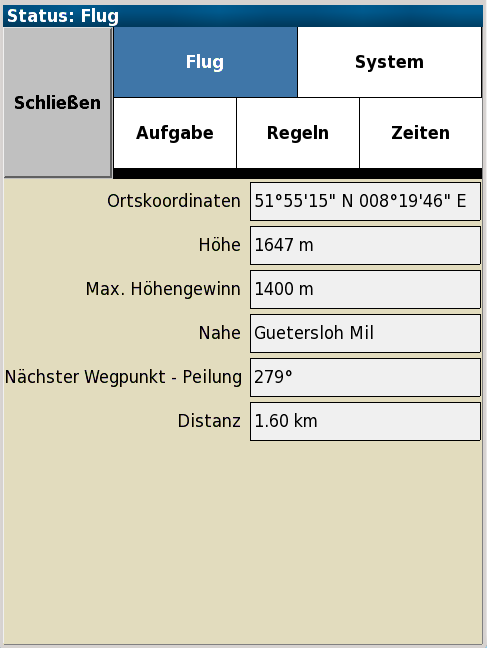
\includegraphics[angle=0,width=0.5\linewidth,keepaspectratio='true']{figures/status-aircraft.png}
%\end{center}

\item[\button{System}] Zeigt den Status von angeschlossenen Geräten, Satellitenempfang,  Batterielevel
%\sketch{figures/status-system.png}
%\begin{center}
%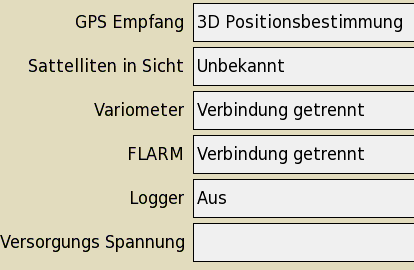
\includegraphics[angle=0,width=0.5\linewidth,keepaspectratio='true']{figures/status-system.png}
%\end{center}

\item[\button{Aufgabe}] Anzeige von AAT-Zeit, Differenz-Zeit, Entfernungen und Aufgabengeschwindigkeit
%\begin{center}
%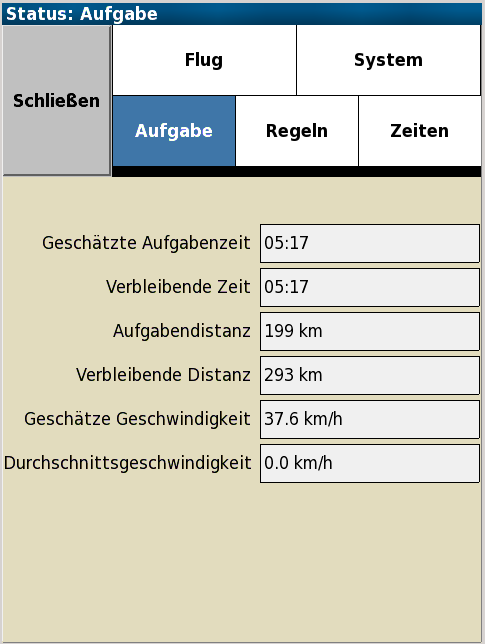
\includegraphics[angle=0,width=0.5\linewidth,keepaspectratio='true']{figures/status-task.png}
%\end{center}

\item[\button{Regeln}] Zeigt Gültigkeit des Abfluges, der Überquerung von Start/Ziellinien gemäß der eingegebenen Regeln der Aufgabe.
%\begin{center}
%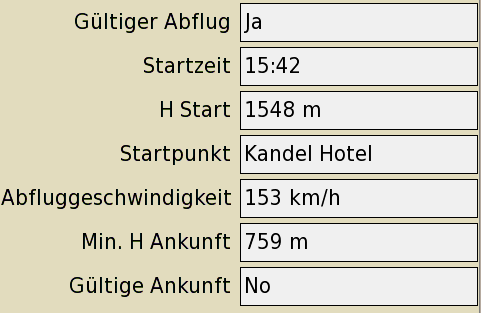
\includegraphics[angle=0,width=0.5\linewidth,keepaspectratio='true']{figures/status-rules.png}
%\end{center}

\item[\button{Zeiten}] Anzeige aller Zeiten wie z.B.: lokale zeit, GPS-zeit, Flugdauer, Start-  und Landezeit sowie den Sonnenuntergang.
%\begin{center}
%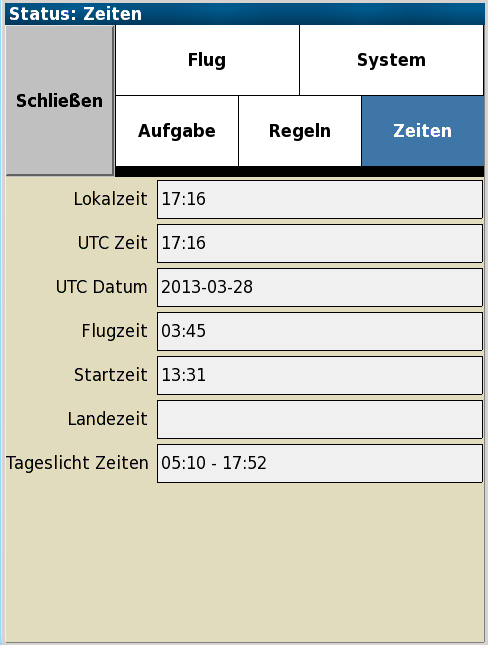
\includegraphics[angle=0,width=0.5\linewidth,keepaspectratio='true']{figures/status-times.png}
%\end{center}
\end{description}

\subsection*{Eingabe von Text} \label{sec:textentry}\index{Texteingabe}\index{Eingabe von Text}

Wie zu erwarten, ist der Texteingabedialog dazu da, Text einzugeben.
Benutzt und aufgerufen wird dieser Dialog von diversen Fenstern und anderen Dialogen, um z.B. Wegpunkte oder TeamCodes  einzugeben, Pilotennamen, Loggerdeklarationen u.v.m\dots
Im Kapitel~\ref{sec:status} wird auf die Details der oben beschriebenen Optionen eingegangen.

\menulabel{\bmenut{Konf.}{2/3}\blink\bmenus{System}} Zwei Möglichkeiten der Eingabe sind möglich und vorgesehen:  "Ranglisten"  und "Tastatur".
Voreingestellt ist "Tastatur"-welche für fast alle Endgeräte\menulabel{\quad\button{Aussehen}\blink\button{Sprache}} -bis auf \al sinnvoller und erheblich schneller und bequemer erscheint. Mit \button{Texteingabestil} wird der gewünschte Stil eingestellt.

Um die entsprechenden  Buchstaben einzugeben, werden im \textit{Ranglisten}-Stil die A+ und  A- Buttons benutzt, drücken auf  \button{$<$} bzw.\   \button{$>$} schiebt den Cursor an die entsprechenden Stelle.
 
\begin{center}
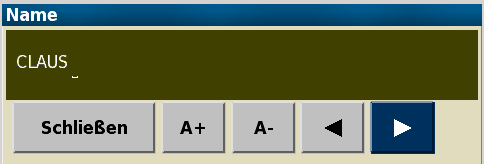
\includegraphics[angle=0,width=0.65\linewidth,keepaspectratio='true']{figures/textentry.png}
\end{center}

Um Text mit dem TouchScreen einzugeben, ist es sinnvoller  auf die "Tastatur"- bzw. Voreinstellung zu wechseln, einfach einen Buchstaben nach dem anderen mit der TouchScreen Tastatur eingeben (s.links).

In einigen Dialogen (z.B. beim Editieren und oder Eingeben \sketch{figures/textentry_keyboard.png}von Wegpunkten) schlägt \textsf{XCSoar} sofort den/die nächsten passenden Einträge aus der Datenbank vor bzw. unterdrückt nicht passende/nicht vorhandene Einträge, sodaß die Eingabe sehr schnell und komfortabel von sich geht.

Um den letzten Buchstaben zu löschen, drücke den  \button{$<-$} button.

Drücke auf  \button{Schließen} um die Eingabe zu übernehmen.

\section{Warntöne}\index{Warntöne}\index{Hinweistöne}

\textsf{XCSoar} erzeugt Geräusche für diverse Ereignisse, welche vom Bediener/Piloten  nach Belieben konfiguriert werden können.
Hierzu siehe~\ref{sec:status} für detaillierte Konfigurierung.

Wenn \textsf{XCSoar} an das VEGA-Variometer angeschlossen ist,  sendet \textsf{XCSoar} Kommando-Strings an das Subsystem des VEGA Sprachsystems, um von diesem Sprachausgaben und Warnungen erzeugen zu lassen, z.B.:

\begin{itemize}
\item Endanflug durch Gelände
\item Anfliegen/erreichen eines Wegpunktes
\item Luftraum Warnungen
\end{itemize}

\section{Bildschirmeinstellungen}

Es können einige Einstellungen der Bildschirmdarstellung und der Details auf \menulabel{\bmenut{Konfig.}{2/3}\blink\bmenus{System}}dem Bildschirm gewählt werden.  Der meistverwendet Punkt  ist hierbei wohl, ob die {\InfoBox}en weiß auf schwarz oder schwarz auf weiß - "invertierte Darstellung" genannt, dargestellt werden \menulabel{\quad\button{Aussehen}\blink\button{Anordnung}}sollen.  Einstellbar über \button{invertierte Infoboxen}. 

Die Einstellung der Helligkeit beim \al erfolgt entweder per \menulabel{\bmenut{Anzeige}{2/2}\blink\bmenus{Helligkeit}}Hardware gemäß des {\em \al User's Manual} oder aber wie links .  




\section{Hilfe System}
  Für die meisten Dialoge ist nun ein Hilfesystem vorhanden.
  Wenn eine Eigenschaft / ein Fenster \menulabel{\bmenus{Hilfe}} aufgerufen wurde, drücke auf den Hilfe-Knopf und eine entsprechender Hilfstext wird erscheinen, der die Auswahlmöglichkeiten  beschreibt. 

\section{Gestures}\label{sec:gestures}\index{Gesten}
Seit Version 6.0 unterstützt \textsf{XCSoar} auch sog.\  "Gesten".

Im Bild links wird angedeutet, wie man sich eine Geste vorzustellen hat. 
Es handelt sich hierbei um eine ganz normale Arbeitsweise, wie sie sie jeder kennt, der mit einem Touchscreen-Gerät
Für den normalen Bildschirm und für den \sketch{figures/gesture1.png} \fl-Bildschirm haben die Gesten unterschiedliche Bedeutungen, wie im  folgender Tabelle beschrieben wird. 
\newpage
 Wenn am Rande folgendes Icon \gesture{Hoch} erscheint, so bedeutet dies, daß für die beschriebene Funktion  die entsprechende Geste verfügbar ist. In diesem Falle  die Geste: ''Hoch''

%Eine Geste wird definiert als eine Bewegung von hoch, runter, rechts und links Bewegungen.
%Die Geste "LU"  z.B.\   steht hierbei für \gesture{Left-Up}.
%(Wenn am Rande der Seite das folgende Icon sichtbar ist, dann  stehen Gesten für die jeweilige Funktion zur %Verfügung.)

\textbf{Auf der Karte verfügbare Gesten:\index{Gesten! auf Karte}}

\begin{itemize}
 \item[\raisebox{-1em}{
\includegraphics[angle=0,width=0.1\linewidth,keepaspectratio='true']{figures/up.png}}] \p{Hoch}: Zoom herein 
 \item[\raisebox{-1em}{
\includegraphics[angle=0,width=0.1\linewidth,keepaspectratio='true']{figures/down.png}}] \p{Runter}: Zoom heraus 
 \item[\raisebox{-1em}{
\includegraphics[angle=0,width=0.1\linewidth,keepaspectratio='true']{figures/left.png}}] \p{Links}: Nächste InfoboxSeite 
 \item[\raisebox{-1em}{
\includegraphics[angle=0,width=0.1\linewidth,keepaspectratio='true']{figures/right.png}}] \p{Rechts}: vorherige InfoboxSeite 
\item[\raisebox{-1em}{
\includegraphics[angle=0,width=0.1\linewidth,keepaspectratio='true']{figures/du.png}}] \p{Runter-Hoch}: Menü anzeigen 
\item[\raisebox{-1em}{
\includegraphics[angle=0,width=0.1\linewidth,keepaspectratio='true']{figures/dr.png}}] \p{Runter-Rechts}: Wegpunkt Dialog anzeigen 
\item[\raisebox{-1em}{
\includegraphics[angle=0,width=0.1\linewidth,keepaspectratio='true']{figures/rd.png}}] \p{Rechts-Runter}: Aufgabenverwaltung
\item[\raisebox{-1em}{
\includegraphics[angle=0,width=0.1\linewidth,keepaspectratio='true']{figures/urdl.png}}] \p{Hoch-Rechts-Runter-links}:  Verschiebemodus.  Dies geht aber auch  auch mit auf Android üblichem Spreizen oder Zusammenfahren von Zeigefinger und Daumen!
\end{itemize}


\textbf{Wenn das \fl-Radar auf dem Bildschirm aktiv ist, sind folgende Gesten verfügbar: }

\index{Gesten!FLARM Radar}
\begin{itemize}
\item[\raisebox{-1em}{
\includegraphics[angle=0,width=0.1\linewidth,keepaspectratio='true']{figures/up.png}}] \p{Hoch}: Zoom herein 
\item[\raisebox{-1em}{
\includegraphics[angle=0,width=0.1\linewidth,keepaspectratio='true']{figures/down.png}}] \p{Runter}: Zoom heraus 
\item[\raisebox{-1em}{
\includegraphics[angle=0,width=0.1\linewidth,keepaspectratio='true']{figures/left.png}}] \p{Links}: Letztes Ziel (Flugzeug)
\item[\raisebox{-1em}{
\includegraphics[angle=0,width=0.1\linewidth,keepaspectratio='true']{figures/right.png}}] \p{Rechts}: Nächstes Ziel (Flugzeug)
\item[\raisebox{-1em}{
\includegraphics[angle=0,width=0.1\linewidth,keepaspectratio='true']{figures/ud.png}}]  \p{Hoch-Runter}: Aktiviere AutoZoom
\item[\raisebox{-1em}{
\includegraphics[angle=0,width=0.1\linewidth,keepaspectratio='true']{figures/dr.png}}] \p{Runter-Rechts}:  Öffne Detail-Fenster des gewählten Zieles (Flugzeuges)
\item[\raisebox{-1em}{
\includegraphics[angle=0,width=0.1\linewidth,keepaspectratio='true']{figures/rd.png}}] \p{Rechts-Runter}:  Öffnet die Aufgabenverwaltung
\item[\raisebox{-1em}{
\includegraphics[angle=0,width=0.1\linewidth,keepaspectratio='true']{figures/rl.png}}] \p{Rechts-Links}: Wechselt zur Anzeige von Werten wie z.B.\ Steigen, relativer Höhe etc.\ des angewählten Zieles (Flugzeuges) )
\end{itemize} 